\begin{figure}[h!]
    \centering
    \setlength{\resLen}{0.5in}
    \setlength{\raiseLen}{0.2in}
    \addtolength{\tabcolsep}{-5pt}
    \scriptsize
    \begin{tabular}{rrlrcc@{\hspace{2\tabcolsep}}lrcc}
    	&
        & \multicolumn{2}{c}{SVBRDF maps} & \multicolumn{2}{c}{Novel views}
        & \multicolumn{2}{c}{SVBRDF maps} & \multicolumn{2}{c}{Novel views}
        \\[2pt]
        & &
        & \raisebox{\raiseLen}{\rotatebox[origin=c]{90}{GT}} &
        \includegraphics[height=\resLen]{svbrdf/results/refine/real_wood-knotty/ref/rendered_nov_1.jpg} &
        \includegraphics[height=\resLen]{svbrdf/results/refine/real_wood-knotty/ref/rendered_nov_2.jpg} &
        & \raisebox{\raiseLen}{\rotatebox[origin=c]{90}{GT}} &
        \includegraphics[height=\resLen]{svbrdf/results/refine/real_cards-blue/ref/rendered_nov_1.jpg} &
        \includegraphics[height=\resLen]{svbrdf/results/refine/real_cards-blue/ref/rendered_nov_2.jpg}
        \\[-1pt]
        & &
        \textit{~~wood-knotty} & &
        \includegraphics[height=0.5\resLen]{svbrdf/results/refine/real_wood-knotty/ref/rendered_nov_1_zoom.jpg} &
        
\includegraphics[height=0.5\resLen]{svbrdf/results/refine/real_wood-knotty/ref/rendered_nov_2_zoom.jpg} &
        \textit{~~cards-blue} & &
        \includegraphics[height=0.5\resLen]{svbrdf/results/refine/real_cards-blue/ref/rendered_nov_1_zoom.jpg} &
        
\includegraphics[height=0.5\resLen]{svbrdf/results/refine/real_cards-blue/ref/rendered_nov_2_zoom.jpg}
        \\[1pt]
        \multirow{4}{*}[0.5\raiseLen]{\rotatebox[origin=c]{90}{No refinement}} &
        \raisebox{\raiseLen}{\rotatebox[origin=c]{90}{Ours}} &
        \multicolumn{2}{c}{\includegraphics[height=\resLen]{svbrdf/results/refine/real_wood-knotty/ours/tex.jpg}} &
        \includegraphics[height=\resLen]{svbrdf/results/refine/real_wood-knotty/ours/rendered_nov_1.jpg} &
        \includegraphics[height=\resLen]{svbrdf/results/refine/real_wood-knotty/ours/rendered_nov_2.jpg} &
        \multicolumn{2}{c}{\includegraphics[height=\resLen]{svbrdf/results/refine/real_cards-blue/ours/tex.jpg}} &
        \includegraphics[height=\resLen]{svbrdf/results/refine/real_cards-blue/ours/rendered_nov_1.jpg} &
        \includegraphics[height=\resLen]{svbrdf/results/refine/real_cards-blue/ours/rendered_nov_2.jpg}
        \\[-1pt]
        & &
        \multicolumn{2}{c}{
\includegraphics[height=0.5\resLen]{svbrdf/results/refine/real_wood-knotty/ours/tex_zoom.jpg}} &
        \includegraphics[height=0.5\resLen]{svbrdf/results/refine/real_wood-knotty/ours/rendered_nov_1_zoom.jpg} &
        
\includegraphics[height=0.5\resLen]{svbrdf/results/refine/real_wood-knotty/ours/rendered_nov_2_zoom.jpg} &
        \multicolumn{2}{c}{
\includegraphics[height=0.5\resLen]{svbrdf/results/refine/real_cards-blue/ours/tex_zoom.jpg}} &
        \includegraphics[height=0.5\resLen]{svbrdf/results/refine/real_cards-blue/ours/rendered_nov_1_zoom.jpg} &
        
\includegraphics[height=0.5\resLen]{svbrdf/results/refine/real_cards-blue/ours/rendered_nov_2_zoom.jpg}
        \\[1pt]
        & \raisebox{\raiseLen}{\rotatebox[origin=c]{90}{[Gao19]+}} &
        \multicolumn{2}{c}{\includegraphics[height=\resLen]{svbrdf/results/refine/real_wood-knotty/msra_egsr/tex.jpg}} &
        \includegraphics[height=\resLen]{svbrdf/results/refine/real_wood-knotty/msra_egsr/rendered_nov_1.jpg} &
        \includegraphics[height=\resLen]{svbrdf/results/refine/real_wood-knotty/msra_egsr/rendered_nov_2.jpg} &
        \multicolumn{2}{c}{\includegraphics[height=\resLen]{svbrdf/results/refine/real_cards-blue/msra_egsr/tex.jpg}} &
        \includegraphics[height=\resLen]{svbrdf/results/refine/real_cards-blue/msra_egsr/rendered_nov_1.jpg} &
        \includegraphics[height=\resLen]{svbrdf/results/refine/real_cards-blue/msra_egsr/rendered_nov_2.jpg}
        \\[-1pt]
        & &
        \multicolumn{2}{c}{
\includegraphics[height=0.5\resLen]{svbrdf/results/refine/real_wood-knotty/msra_egsr/tex_zoom.jpg}} &
        \includegraphics[height=0.5\resLen]{svbrdf/results/refine/real_wood-knotty/msra_egsr/rendered_nov_1_zoom.jpg} &
        
\includegraphics[height=0.5\resLen]{svbrdf/results/refine/real_wood-knotty/msra_egsr/rendered_nov_2_zoom.jpg} &
        \multicolumn{2}{c}{
\includegraphics[height=0.5\resLen]{svbrdf/results/refine/real_cards-blue/msra_egsr/tex_zoom.jpg}} &
        \includegraphics[height=0.5\resLen]{svbrdf/results/refine/real_cards-blue/msra_egsr/rendered_nov_1_zoom.jpg} &
        
\includegraphics[height=0.5\resLen]{svbrdf/results/refine/real_cards-blue/msra_egsr/rendered_nov_2_zoom.jpg}
        \\[1pt]
        \hline\\[-6pt]
        \multirow{4}{*}[0.5\raiseLen]{\rotatebox[origin=c]{90}{With refinement}} &
        \raisebox{\raiseLen}{\rotatebox[origin=c]{90}{Ours}} &
		\multicolumn{2}{c}{\includegraphics[height=\resLen]{svbrdf/results/refine/real_wood-knotty/ours+/tex.jpg}} &
		\includegraphics[height=\resLen]{svbrdf/results/refine/real_wood-knotty/ours+/rendered_nov_1.jpg} &
		\includegraphics[height=\resLen]{svbrdf/results/refine/real_wood-knotty/ours+/rendered_nov_2.jpg} &
		\multicolumn{2}{c}{\includegraphics[height=\resLen]{svbrdf/results/refine/real_cards-blue/ours+/tex.jpg}} &
		\includegraphics[height=\resLen]{svbrdf/results/refine/real_cards-blue/ours+/rendered_nov_1.jpg} &
		\includegraphics[height=\resLen]{svbrdf/results/refine/real_cards-blue/ours+/rendered_nov_2.jpg}
		\\[-1pt]
		& &
		\multicolumn{2}{c}{
\includegraphics[height=0.5\resLen]{svbrdf/results/refine/real_wood-knotty/ours+/tex_zoom.jpg}} &
		\includegraphics[height=0.5\resLen]{svbrdf/results/refine/real_wood-knotty/ours+/rendered_nov_1_zoom.jpg} &
		
\includegraphics[height=0.5\resLen]{svbrdf/results/refine/real_wood-knotty/ours+/rendered_nov_2_zoom.jpg} &
		\multicolumn{2}{c}{
\includegraphics[height=0.5\resLen]{svbrdf/results/refine/real_cards-blue/ours+/tex_zoom.jpg}} &
		\includegraphics[height=0.5\resLen]{svbrdf/results/refine/real_cards-blue/ours+/rendered_nov_1_zoom.jpg} &
		
\includegraphics[height=0.5\resLen]{svbrdf/results/refine/real_cards-blue/ours+/rendered_nov_2_zoom.jpg}
		\\[1pt]
        & \raisebox{\raiseLen}{\rotatebox[origin=c]{90}{[Gao19]+}} &
        \multicolumn{2}{c}{\includegraphics[height=\resLen]{svbrdf/results/refine/real_wood-knotty/msra+_egsr/tex.jpg}} &
        \includegraphics[height=\resLen]{svbrdf/results/refine/real_wood-knotty/msra+_egsr/rendered_nov_1.jpg} &
        \includegraphics[height=\resLen]{svbrdf/results/refine/real_wood-knotty/msra+_egsr/rendered_nov_2.jpg} &
        \multicolumn{2}{c}{\includegraphics[height=\resLen]{svbrdf/results/refine/real_cards-blue/msra+_egsr/tex.jpg}} &
        \includegraphics[height=\resLen]{svbrdf/results/refine/real_cards-blue/msra+_egsr/rendered_nov_1.jpg} &
        \includegraphics[height=\resLen]{svbrdf/results/refine/real_cards-blue/msra+_egsr/rendered_nov_2.jpg}
        \\[-1pt]
        & &
        \multicolumn{2}{c}{\includegraphics[height=0.5\resLen]{svbrdf/results/refine/real_wood-knotty/msra+_egsr/tex_zoom.jpg}} &
        \includegraphics[height=0.5\resLen]{svbrdf/results/refine/real_wood-knotty/msra+_egsr/rendered_nov_1_zoom.jpg} &
        \includegraphics[height=0.5\resLen]{svbrdf/results/refine/real_wood-knotty/msra+_egsr/rendered_nov_2_zoom.jpg} &
        \multicolumn{2}{c}{\includegraphics[height=0.5\resLen]{svbrdf/results/refine/real_cards-blue/msra+_egsr/tex_zoom.jpg}} &
        \includegraphics[height=0.5\resLen]{svbrdf/results/refine/real_cards-blue/msra+_egsr/rendered_nov_1_zoom.jpg} &
        \includegraphics[height=0.5\resLen]{svbrdf/results/refine/real_cards-blue/msra+_egsr/rendered_nov_2_zoom.jpg}
    \end{tabular}
    \caption[Per-pixel post-refinement]{\label{fig:svbrdf:refine}
        \small \textbf{Per-pixel post-refinement.} Unlike Gao's method, post-refinement via per-pixel optimization makes less of a difference in our method.
        Without post-refinement, [Gao19]+ (i.e., Gao's method initialized with Deschaintre's \cite{Deschaintre2019} direct predictions) usually produces blurry results, as shown in the row marked as ``[Gao19]+ (NR)''.
        Our method, on the contrary, does not rely nearly as heavily on post-refinement: Without it, our results are already quite sharp (see ``Ours (NR)''), thanks to the generative power of our MaterialGAN.
        A zoomed-in version is attached below each SVBRDF map and novel-view image.
    }
\end{figure}
